\documentclass[12pt, letterpaper]{article}

\usepackage{graphicx}
\graphicspath{ {images/} }

%opening
\title{Neural Network Classification of Privacy Policy Data Practices}
\author{Dr. Noriko Tomuro, August Karlstedt}

\begin{document}

\maketitle

\begin{abstract}
Privacy policies and the practices outlined in them impact every user to a given website. These policies usually include descriptions of the practices that the website operators use to collect, share, and use user data. Often unread by users because of their length and technical detail, users are unaware of how and where their data is being analyzed. We use the OPP-115 corpus of 115 privacy policies to train a neural network to classify text spans into one of ten categories in an effort to simplify these policies.
\end{abstract}

\section{Introduction}
The OPP-115 corpus is a collection of privacy policies that have been manually annotated \cite{wilson2016creation}. These annotations are a range of characters with an associated category. The possible categories include:

\begin{itemize}
\item First Party Collection/Use: how and why a service provider collects user information.
\item Third Party Sharing/Collection: how user information may be shared with or collected by third parties.
\item User Choice/Control: choices and control options available to users.
\item User Access, Edit, \& Deletion: if and how users may access, edit, or delete their information.
\item Data Retention: how long user information is stored.
\item Data Security: how user information is protected.
\item Policy Change: if and how users will be in formed about changes to the privacy policy.
\item Do Not Track: if and how Do Not Track signals 3 for online tracking and advertising are honored.
\item International \& Specific Audiences: practices that pertain only to a specific group of users (e.g., children, Europeans, or California residents).
\item Other: additional sublabels for introductory or general text, contact information, and practices not covered by the other categories.
\end{itemize}

These categories were determined by domain experts (privacy experts, public policy experts, legal scholars) in Sadeh et al. 2016. We use these categories as our target variables for our network, which we later describe in further detail. Since these categories encompass a wide range of practices, a summary of a given privacy policy could be generated with them, helping users understand its contents.

\section{Related Work}
TODO

\section{Data Preparation}
The OPP-115 corpus includes annotated 115 annotated policies, each with sub-categories. In this work, we only inspect the 10 higher-level categories. 

To prepare the data for the network, we encode the 10 data practice categories into one hot encoded representations.  

For the text spans, we take some normalization and preprocessing steps. First, we convert the text to lowercase. We then apply the Natural Language Toolkit (NLTK) lemmatizer. With the resulting processed text span, we build a vocabulary for a Paragraph2Vec model.

In the above proprocessing steps, we also keep track of the selected text spans in a given policy in order to generate an eleventh category for "None" -- a category where a given text span could relate to none of the possible data practices.

Finally, we train gensim's implementation of a Paragraph2Vec model on the text spans from our corpus, along with the unselected text spans that we have generated for 16 epochs.

This results in the following examples for each category:
\begin{itemize}
\item 942 Data Retention
\item 1008 Data Security
\item 90 Do Not Track
\item 37299 First Party Collection/Use
\item 937 International and Specific Audiences
\item 3544 Other
\item 1225 Policy Change
\item 25024 Third Party Sharing/Collection
\item 1691 User Access, Edit and Deletion
\item 6146 User Choice/Control
\item 1764 None
\end{itemize}

\section{Network Setup}
The artificial neural network built here is constructed using the Keras library. Our network consists of the following layers:

\begin{itemize}
\item Fully connected layer with 256 nodes, ReLU activation
\item Dropout 25\% of the inputs
\item Fully connected layer with 256 nodes, ReLU activation
\item Dropout 25\% of the inputs
\item Fully connected layer with 11 nodes, Softmax activation
\end{itemize}

Softmax is used to produce probability distributions between the 11 possible categories and ReLU activations are Rectified Linear Units. 

Dropout is used to prevent overfitting of the training data.

We train for 128 epochs on minibatches of size 128, with a validation split of 25\%, resulting in a training set size of 59752 samples and a validation set size of 19918 samples.

\section{Results}
Results before adding the \textit{None} category were significantly better. 

\textbf{TODO: Describe them here.}

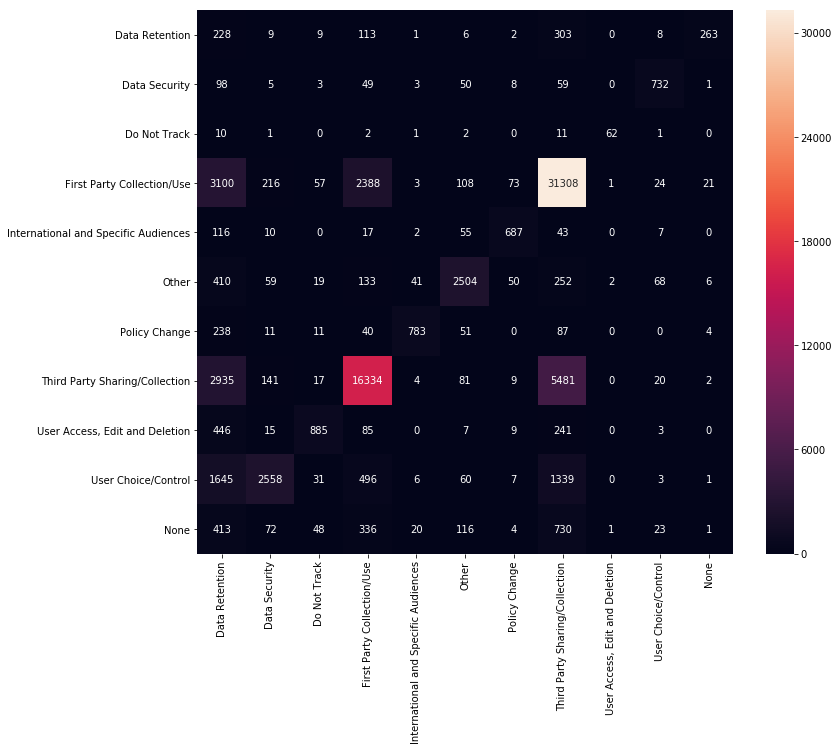
\includegraphics[width=\linewidth]{confusion-matrix}

Current results across all 11 categories results in a accuracy of 77.01\% on the training data and 51.75\% on the validation data. It is evident that the network is overfitting the training data and not learning a good representation for the mapping of training example to target. Further improvements are described in the next section.

\section{Future Work}
\begin{itemize}
\item Tweak the parameters for training the Paragraph2Vec model, e.g. number of epochs, dimensionality
\item Refine the neural network architecture
\item Perform hyperparameter tuning
\item Ensure that the text spans of the \textit{None} category do not overlap with other text spans
\item Input entire sentence or paragraph boundaries instead of just the selected text span
\item Modify the network to take advantage of recurrent neural networks since text is a sequence. It may imrpove learning of the relationships between words and categories.
\end{itemize}

\newpage
\bibliographystyle{ieeetr}
\bibliography{bibliography} 


\end{document}
